%----------------------------------------------------------------------------
\chapter{Models}\label{sect:Models}
%----------------------------------------------------------------------------
\section{Encode Process Decode model}
This model has been tested and used in the demos provided on GitHub.
\begin{figure}[!ht]
	\centering
	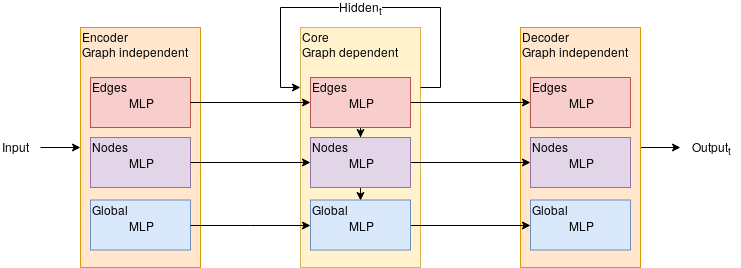
\includegraphics[width=150mm, keepaspectratio]{figures/EPD.png}
	\caption{Representation of the model.}
	\label{fig:encode-process-decode}
\end{figure}

As it is shown on the Figure~\ref{fig:encode-process-decode} above the model consist of 3 different parts.

\subsection{Encoder}
The encoder model is a graph independent model that uses multi layer perceptrons and layer normalization on the global attributes, the edge feature vectors and the node feature vectors. There are not shared variables between the multi layer perceptrons.

\subsection{Core}
This is the only graph dependent part of the model. It also uses multi layer perceptrons and layer normalization as the previous one, but the graph dependency enables it to use the predicted edge features to influence the node features and these impact the global feature.

This section of the network is repeated resulting in a hidden state that gets feed forward again in the Core section. Each step has its own output with its timestamp.

\subsection{Decoder}
The decoder model has the same structure as the encoder. It does not use any kind of activation on the last layer, which enables it to better generalization, but also making it harder to use on a specific project eq. classifying whether or not the summary graph contains the given node or edge.

\section{GraphAttention model - first iteration}
This model is highly inspired by the Encode Process Decode model, but it is better suited for NLP problems as you can see on Figure~\ref{fig:graph-attention0}.

\begin{figure}[!ht]
	\centering
	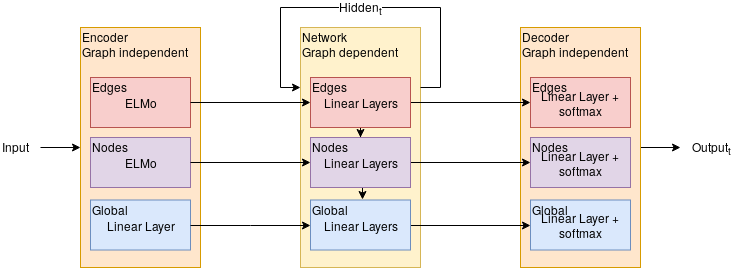
\includegraphics[width=150mm, keepaspectratio]{figures/GA0.png}
	\caption{Representation of the model.}
	\label{fig:graph-attention0}
\end{figure}

\subsection{Encoder}

The encoder is made up of two Embedding layers one for the nodes' lemmas and one for the edges' relation type (See Figure~\ref{fig:graph-attention0-encoder}). The second one's necessity is questionable, since it does not contain as much information and could be also represented with a simple one-hot encoded vector, since it has not as high dimensionality as the nodes. However I decided I leave it in the model and make it a changeable parameter of the network.

\begin{figure}[!ht]
	\centering
	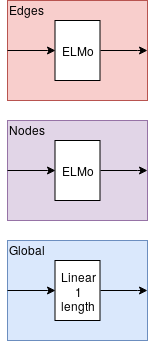
\includegraphics[scale=0.5]{figures/GA0_encoder.png}
	\caption{Representation of the encoder part of the model.}
	\label{fig:graph-attention0-encoder}
\end{figure}

For the global features I only used a simple linear layer without activation functions, since it does not need to be encoded in any way.

All of these blocks work independently from each other.

\subsection{Network}

The Network, or core part of the model consists of activated linear layers with differing sizes as depicted on Figure~\ref{fig:graph-attention0-network}.

\begin{figure}[!ht]
	\centering
	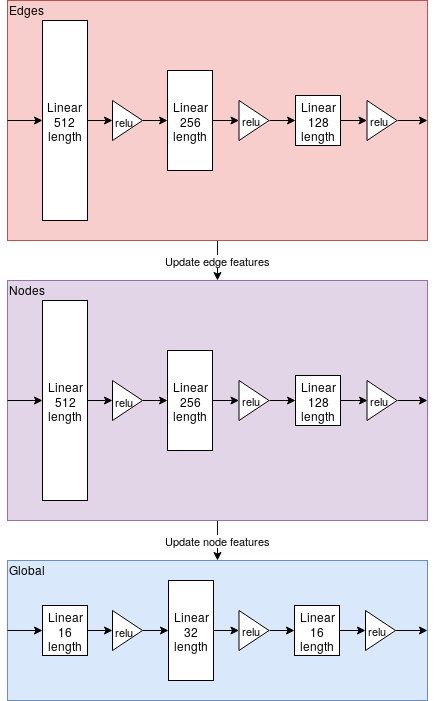
\includegraphics[scale=0.5]{figures/GA0_network.png}
	\caption{Representation of the network part of the model.}
	\label{fig:graph-attention0-network}
\end{figure}

\subsection{Decoder}

\begin{figure}[!ht]
	\centering
	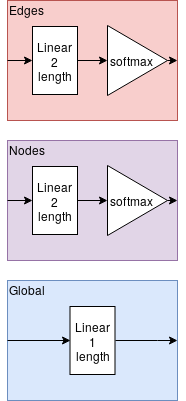
\includegraphics[scale=0.5]{figures/GA0_decoder.png}
	\caption{Representation of the decoder part of the model.}
	\label{fig:graph-attention0-decoder}
\end{figure}